\documentclass[12pt]{article}
\usepackage[english]{babel}
\usepackage[utf8x]{inputenc}
\usepackage[T1]{fontenc}
\usepackage{scribe}
\usepackage{listings}
\usepackage{fullpage}
\usepackage{amsfonts}
\usepackage{amssymb}
\usepackage{url}

\usepackage[svgnames]{xcolor}
\usepackage{color}
% \definecolor{light-gray}{gray}{0.90}
% \lstset{backgroundcolor=\color{light-gray},showlines=true}

% \usepackage{xcolor}
% \usepackage{listings}

% \lstdefinestyle{BashInputStyle}{
%   language=bash,
%   basicstyle=\small\sffamily,
%   numbers=left,
%   numberstyle=\tiny,
%   numbersep=3pt,
%   frame=tb,
%   columns=fullflexible,
%   backgroundcolor=\color{yellow!20},
%   linewidth=0.9\linewidth,
%   xleftmargin=0.1\linewidth
% }


\usepackage{minted}
\setminted{fontsize=\footnotesize,baselinestretch=0.5}

\Scribe{}
\Lecturer{Queenie Qiu, John Raiti. Student: \textbf{Shucheng Guo}}
\LectureNumber{1}
\LectureDate{DATE: Jan 12th. 2023}
\LectureTitle{Sensors in ROS}

\lstset{style=mystyle}

\begin{document}
	\MakeScribeTop

%#############################################################
%#############################################################
%#############################################################
%#############################################################
 

\section {Gazebo introduction}
Gazebo is a high-fidelity 3D simulator stemming from the need to
simulate robots in various environments and conditions.
Execute the following line in a terminal:

\begin{minted}{bash}
  $ roslaunch gazebo_ros empty_world.launch world_name:=worlds/cafe.world
\end{minted}

As you may see in this example, Gazebo simulates a cafe with different objects, from simple shapes to complex models that are governed by dynamic and static properties as well as physics constraints. Now let’s add a robot. 

\subsection{Spawning a robot in Gazebo}

This method uses a small python script called spawn\_model to make a service call request to the gazebo\_ros ROS node (named simply "gazebo" in the rostopic namespace) to add a custom URDF into Gazebo. The spawn\_model script is located within the gazebo\_ros package. Open a new termianl and use this script in the following way:
\begin{minted}{bash}
  $ roscd turtlebot3_description/urdf/
  $ rosrun gazebo_ros spawn_model -urdf -file turtlebot3_burger.urdf.xacro
  
   -x 0 -y 0 -z 1 -model TURTLEBOT3_MODEL 
\end{minted}

\textbf{Note}: Normally, we can take advantage of the roslaunch command as we are loading the gazebo world, and add the robot spawning portion to the launch file. The resulting added code would look like the following lines:
\begin{figure}[H]
  \vspace{-10pt}
  \centering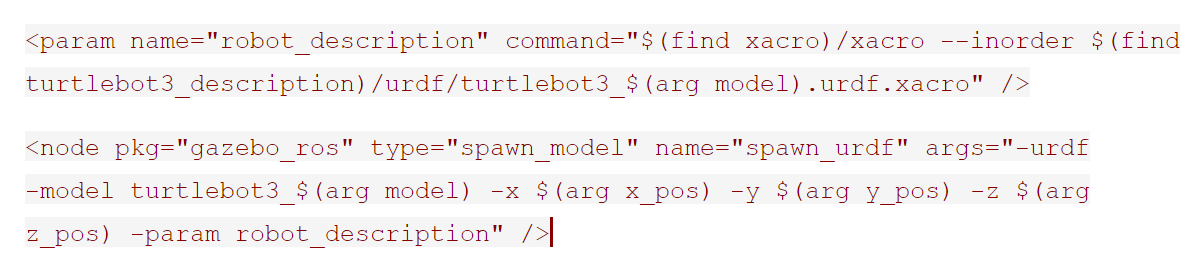
\includegraphics[width=14cm]{lab1figure/lab1gazebo.png}\vspace{-10pt}
  \caption{illustration of the launch file.}\label{fig:omni}
  \end{figure}

\subsection{Creating object models in Gazebo}
\begin{enumerate}
    \item You can add additional objects and shapes into your simulated environment. On the top of the right panel, click on the cylinder shape to add a pillar object into the world. When you right-click on the object you can modify its properties, like dimension and the collision area. Select edit model, the open link inspector. In both the visual and collision tabs, add the following dimensions in the Geometry section: radius = 0.25m, length = 1m. An illustration is shown below:
    
\begin{figure}[H]
  \vspace{-10pt}
  \centering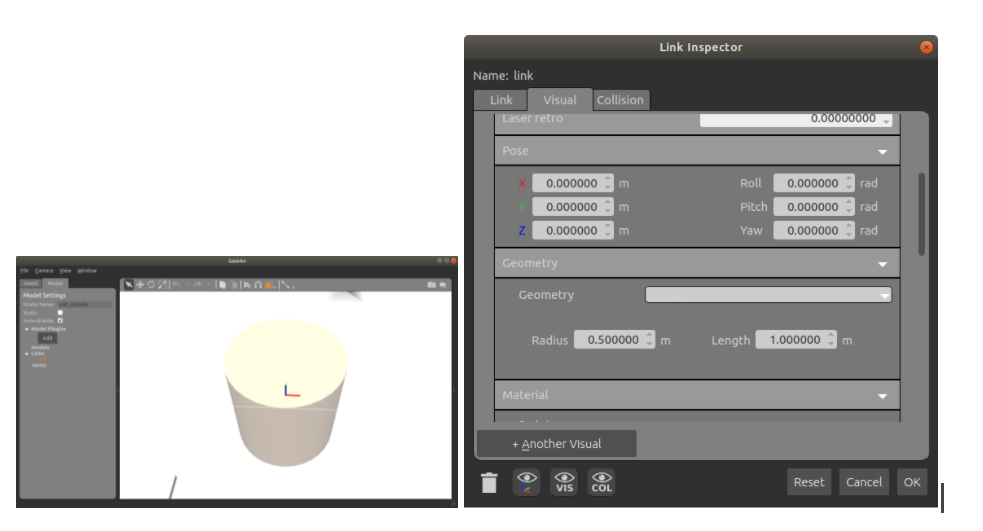
\includegraphics[width=14cm]{lab1figure/lab1gazebodemo.png}\vspace{-10pt}
  \caption{An illustration of creating a model in gazebo.}\label{fig:omni1}
  \end{figure}
    
    \item Once you have created your pillar model, you can save it (full path:\\ ~/catkin\_ws/src/turtlebot3\_simulations/turtlebot3\_gazebo/models). This will allow you to insert the object with its customized properties in new worlds. If you open this folder you will see a new folder called like the object you created, and it will contain two files: model.config and model.sdf
\end{enumerate}

\textbf{Deliverable: Take a screenshot of the modified cafe.world with your pillar in it.}

\begin{figure}[H]
  \centering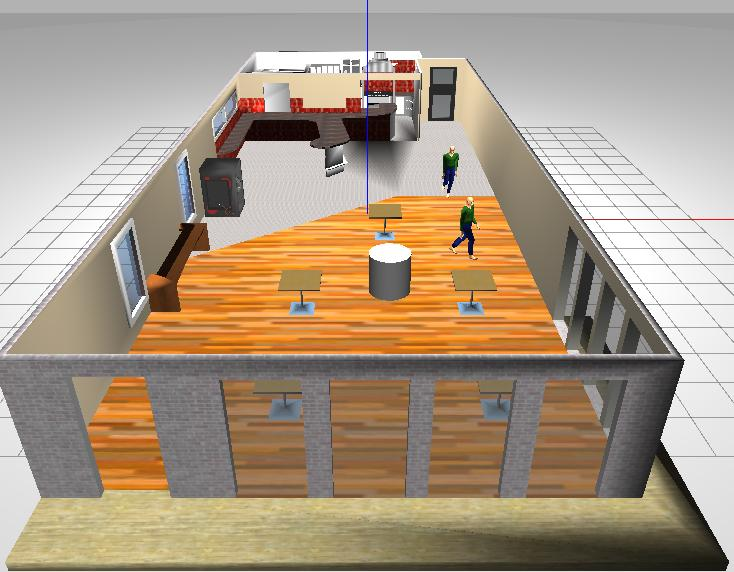
\includegraphics[width=14cm]{lab1figure/mod_pillar.jpg}\vspace{-10pt}
  \caption{Modifying \mintinline{bash}{cafe.world} with a pillar.}\label{fig:mod_pillar}
  \end{figure}

\section{Setting up the working environment}
First, we want to set up the simulation environment to work with the turtlebot3. We will be using a simple world with four walls where the turtlebot3 burger can interact.
\begin{enumerate}

\item Select the turtlebot3 model to be burger and use the 'roslaunch' command to spawn a gazebo world with a turtlebot3 in it. 
\begin{minted}{bash}
  $ export TURTLEBOT3_MODEL=burger
  $ roslaunch turtlebot3_gazebo turtlebot3_stage_1.launch
\end{minted}

\item Open a new terminal and try to visualize the robot and its sensors in RViz. 

\begin{minted}{bash}
  $ rviz rviz
\end{minted}

\item Then click on the add button, select RobotModel and add it to the RViz panel.

Note: At this point, you will find errors related to failure to map from odom to base\_link, wheel\_right, wheel\_left.
If you take a closer look at the launch file for the gazebo world, and inspect what nodes are brought up by it, you will realize that the robot that has been spawned is only the footprint of one. To interact with variables like velocity of sensor information, we need to bring up all the necessary topics and nodes through the robot\_state\_publisher.

\item In another terminal, type the following command to visualize the transforms tree. You will notice there is only a transformation between the /odom reference frame and the /base\_footprint. The latter represents the point on the floor where the robot is supposed to occupy.

\begin{minted}{bash}
  $ rosrun rqt_tf_tree rqt_tf_tree
\end{minted}

\item In a new terminal you will bring up a full robot model with all its transformations. 

\begin{minted}{bash}
  $ roslaunch turtlebot3_bringup turtlebot3_remote.launch
\end{minted}

After that, you can retry the rqt\_tf\_tree command and expect to see the following:
\begin{figure}[H]
  \vspace{-10pt}
  \centering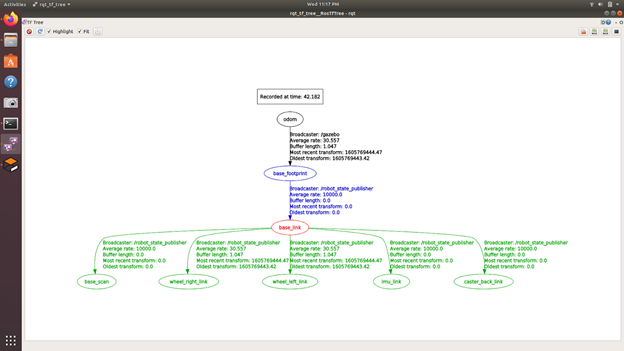
\includegraphics[width=14cm]{lab1figure/rqf.png}\vspace{-10pt}
  \caption{rqt\_tf\_tree.}\label{fig:rqt}
  \end{figure}

\textbf{Note}: If your rviz visualization has no robot, you can change the fixed frame to "odom", at this point the robot should be visualized in RViz.
\begin{figure}[H]
  \vspace{-10pt}
  \centering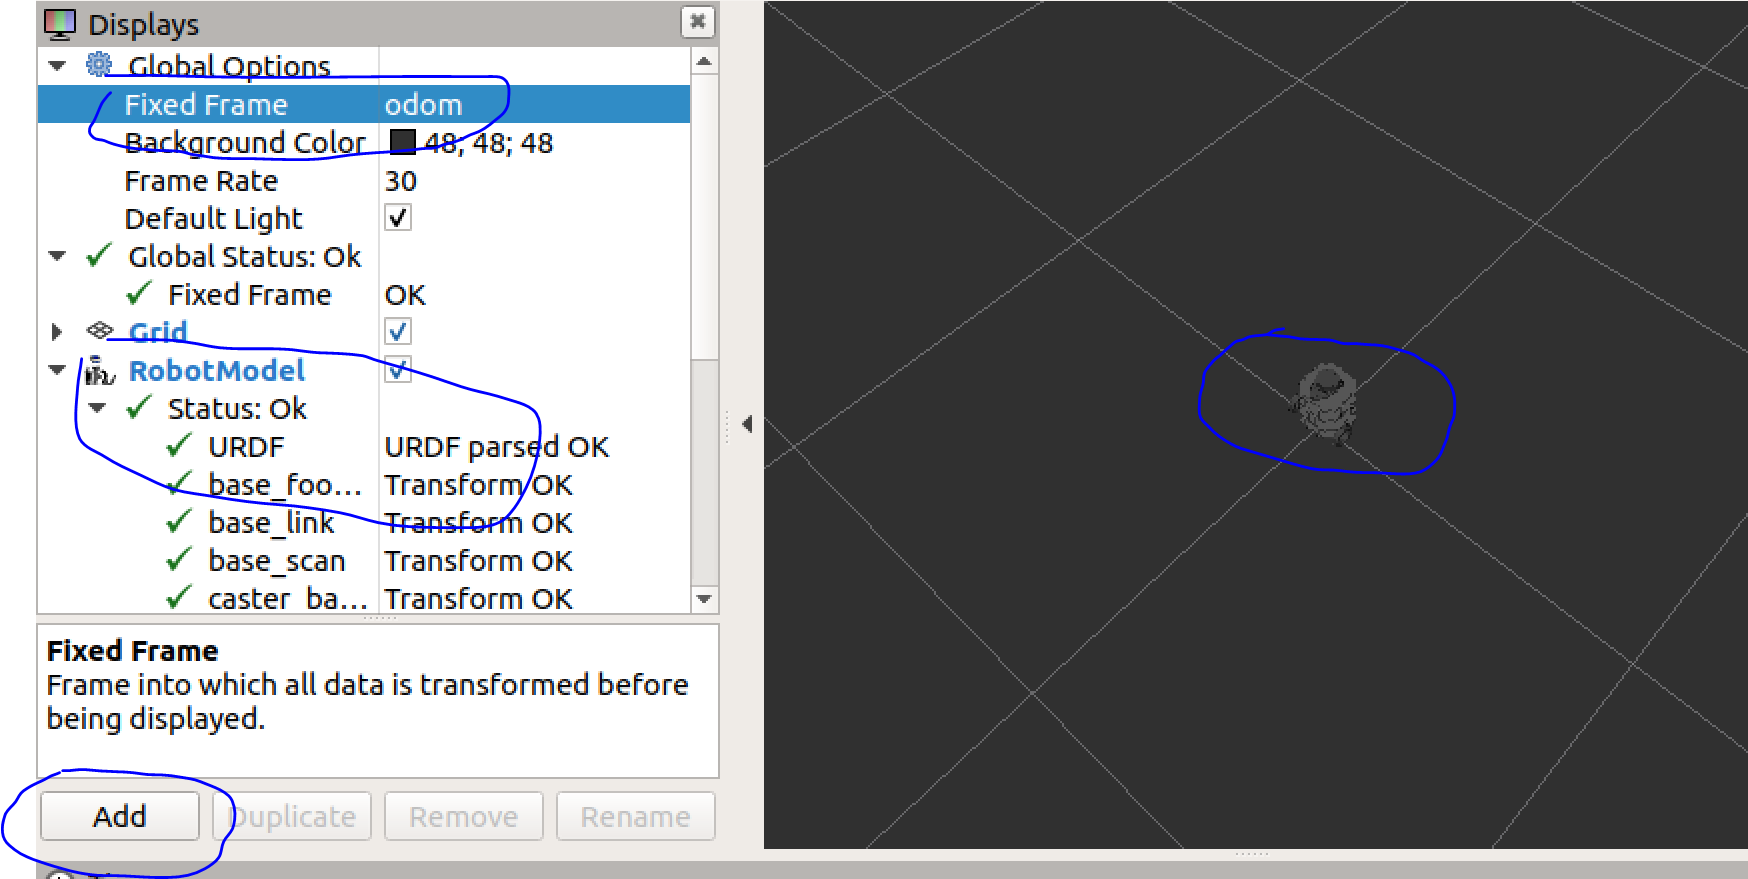
\includegraphics[width=14cm]{lab1figure/rviz.png}\vspace{-10pt}
  \caption{rviz visualization.}\label{fig:rqt1}
  \end{figure}

Now that the robot is fully brought up and functioning in simulation, we will go through the examples available with the turtlebot3 package.

\end{enumerate}

\section{Running turtlebot3 examples}
You have spawned the robot in a Gazebo simulation, just in case you closed them, you need to open two terminals and type:\\

For one terminal:
\begin{minted}{bash}
  $ roslaunch turtlebot3_gazebo turtlebot3_stage_1.launch
\end{minted}

For another terminal:

\begin{minted}{bash}
  $ roslaunch turtlebot3_bringup turtlebot3_remote.launch
\end{minted}

Then explore the different examples available from the turtlebot3 metapackage. Additional information can be found in this link:

% \url{https://emanual.robotis.com/docs/en/platform/turtlebot3/basic\_examples/\basic-examples}

\begin{enumerate}
  \item Move using Interactive Markers: this example uses input coming from rviz. An overlayed marker consisting of arrows and a ring surrounding the robot’s position are used to modify the cmd\_vel topic with linear and angular velocity changes. \textbf{Note}: you need to add the interactive markers to the panel.

  \begin{minted}{bash}
    $ roslaunch turtlebot3_example interactive_markers.launch

    $ rosrun rviz rviz -d `rospack find turtlebot3_example`/rviz
    /turtlebot3_interactive.rviz
  \end{minted}

  As you manipulate the interactive markers in rviz, you may be able to use new terminals to inspect the active nodes and topics (through rqt\_graph) or to echo the changes done to the cmd\_vel topic (rostopic echo /cmd\_vel) as you visualize both in rviz and gazebo the result of these interactions.

  \textbf{Deliverables}: 

    \begin{enumerate}

      \item Take a screenshot of the resulting rqt\_graph.
    
      \begin{figure}[H]
        \centering
\includegraphics[width=14cm]{lab1figure/rosgraph.png}\vspace{-10pt}
        \caption{Resulting \mintinline{bash}{rqt} graph.}\label{fig:rosgraph}
        \end{figure}

      \item What information is flowing between the nodes?

      \textbf{Answer: }Velocity and direction changes in the topic \mintinline{bash}{/cmd_vel} are the information exchanged between the nodes.

      \item Describe, in detail, what this information is used for within the robot.
    
      \textbf{Answer: }The information show linear (x, y) and angular (z) changes in both direction and velocity. 
      Positive values in x and y drive the robot forward, while those in z to the left; negative values in x and y drive the robot backward, while z to the right.
      Values indicate the magnitude of the velocity change, in the unit of meters per second.
    
      \item Describe the resulting behavior of the robot when you use either the arrows or the ring on the interactive marker. Copy one of the echo messages for velocity.
    
      \textbf{Answer: }Velocity only changes in one plane if only the arrow or the thing is pressed, meaning there is only one non-zero value on x, y and z axes. For one click on the arrow, the echoed messages are shown below:

      \begin{minted}[baselinestretch=1.2]{bash}
        linear:
          x: -0.005202962551265955
          y: 0.0
          z: 0.0
        angular:
          x: 0.0
          y: 0.0
          z: 0.0
      \end{minted}

    \end{enumerate}

  \item Point Operation: in this example the user specifies an input corresponding to x | y | z. The first two numbers are distance numbers and the third is an angle value ( -180 to 180), referenced to the world origin in Gazebo (the robot spawned in the origin (0 | 0 | 0). The symbol | represents a space bar character, a correct command for the robot would be “1 1 90”.

  \begin{minted}{bash}
    $ roslaunch turtlebot3_example turtlebot3_pointop_key.launch
  \end{minted}

  Tip: You can reset the robot’s position to its original pose in Gazebo:\\
  Edit -> Reset Model Poses (Ctrl + Shift + R)

  \textbf{Deliverables}:

  \begin{enumerate}

      \item Give the robot a command to reach the point x: 1 y: 1.5 w: -90. Describe how the robot is reaching the goal and what do you observe while watching the robot. Does it match position and orientation at the same time? Or does it do it in a specific sequence?
      
      \textbf{Answer: }To reach the goal of \mintinline{bash}{(1, 1.5, -90)}, from the top view, the robot walks 1.5 units left and 1 up to its northwest, and then turns 90 degrees, facing east.
      \\After receiving the command, the robot walks to the designated point \mintinline{bash}{(x, y)} before it turns the direction toward that described in \mintinline{bash}{z}.

      \item Edit the initial position of the robot to be different from the origin (x:0 y:0 w:0) using the Gazebo interface. Run the same command as before to reach the point x:1 y:1.5 w:-90.
      
      \begin{enumerate}
          \item Describe the motion of the robot and with respect to which reference frame (the world’s on Gazebo or its own reference frame).
          
          \textbf{Answer: }The origin of the robot is set to \mintinline{bash}{(-1, -1.5)}, which is 1.5 units right and 1 down. The goal is \mintinline{bash}{(1, 1.5)}, which is 1.5 units left and 1 up from \mintinline{bash}{(0, 0)}.
          \\To reach the destination, the robot walks 3 units left and 2 up to the same point as in the last question, and then turns east.

          \item Determine the transformation between the Gazebo origin and the robot’s new initial position. How would the instruction look (x: <value> y: <value> w: <value>) if it was from the robot’s own reference frame.
          Tip: you can use vector representation or a diagram.

          \textbf{Answer: }As explained in the last answer, the robot walks left for 3 units and up for 2, while rotating the same angle.
          \\From its own reference frame, the instruction would be \mintinline{bash}{(x: 2, y: 3, z: -90)}.

          \item Discuss the relevance of absolute and relative transformations.
          
          \textbf{Answer: }Absolute transformation is the positional and angular change from the Gazebo origin \mintinline{bash}{(0, 0, 0)}, which relative transformation is one compared to the robot's initial position.
          \\The coordinates we command to transform are absolute transformations, as they're relative to the Gazebo origin; the relative one is calculated based on two transformations, current and final.
          \\They are not necessarily related, but the calculation of the relative transformation involves the absolute transformations.

      \end{enumerate}

  \end{enumerate}

  \item Patrol: this example requires to run two nodes, a server and a client. The client can run through roslaunch; the server node through the rosrun command. In the client terminal, the user can specify a command to determine the mode of patrol (square, triangle, circle), the distance parameter (side or radius), and the number of cycles in the patrol pattern.

  \begin{minted}{bash}
    $ roslaunch turtlebot3_example turtlebot3_client.launch

    $ rosrun turtlebot3_example turtlebot3_server
  \end{minted}

  \textbf{Note}: These patrolling movements are performed using odometry information to know how much the robot has moved. Notice the accumulation of inaccuracy in the patrol shape as the distances or the number of cycles are larger.

  \textbf{Tip}: In the event of colliding with the environment in Gazebo, you can reset the robot’s position Edit -> Reset Model Poses (Ctrl + Shift + R)

  \textbf{Deliverables:}
  
  \begin{enumerate}

    \item Inspect the code for the turtlebot3\_server node:
    
    \begin{enumerate}
    
      \item What are the topics used in the subscribers of the code and what are the message types?
    
        \begin{enumerate}
          \item Topic: \mintinline{bash}{joint_states} Type: \mintinline{bash}{JointState};
          \item Topic: \mintinline{bash}{odom} Type: \mintinline{bash}{Odometry};
        \end{enumerate}

      \item Where is the data used in the code?
    
      \textbf{Answer: }All of the three arguments are passed in an instance of the class object \mintinline{bash}{Turtlebot3Action}.
      \\The patrol mode \mintinline{bash}{mode} and the distance parameter \mintinline{bash}{area} are both called in the method \mintinline{bash}{execute_cb}.
      \\The number of cycles to move \mintinline{bash}{count} is called in the method \mintinline{bash}{go_front}.

    \end{enumerate}

    \item Describe how the code can perform different shapes (turn different angles). How is the information from the sensors used?
    
    \textbf{Answer: }By passing the \mintinline{bash}{mode} argument that specifies the patrol pattern, we can determine the robot's angles in motion. Square is \mintinline{bash}{s}, Triangle \mintinline{bash}{t} and Circle \mintinline{bash}{c}.
    \\Odometry information is passed in and recorded by the method \mintinline{bash}{get_odom}, and then converted to the current position, with which the last movement is calculated, by the method \mintinline{bash}{get_state}.
  
  \end{enumerate}

\end{enumerate}

\section{Sensors}
In this section, we will take a closer look at the information coming from odometry and the LiDAR sensor. We will use the patrol example and create a node which subscribes to the /odom topic to plot the position of the robot throughout the patrol behavior. Additionally, we will create a new node that subscribes to the /scan topic, and moves the robot towards an object that is close by.

\subsection{Creating nodes to visualize sensor data from the odometry topic}

Create a node to subscribe to the odometry topic to create an x-y plot of the robot’s reported position. You will find a plot\_odom.py file in the lab1 folder. This code is currently incomplete. You will need to fill out the TODOs to make it work. You may need to move the file to a ros package (recommended turtlebot3\_examples/nodes) and make the file to be executable before rosrunning it (using the chmod +x command in the terminal). 
\\
\textbf{Tip}: You may need to install the necessary packages to run the plot\_odom.py file correctly.

\begin{minted}{bash}
  $ sudo apt install python-numpy python-matplotlib
\end{minted}

\textbf{Deliverables:}

\begin{enumerate}

    \item Run your patrol example to complete one cycle of 1m square. (the parameters to fill in the client program would be: s 1 1)
    
    \begin{enumerate}

        \item Describe the behavior of the robot in terms of inaccuracies associated with the odometry. What do you observe about the ending position and orientation of the robot?
        
        \textbf{Answer: }The robot deviates from its path of patrol after making turns, and walking distances. The more cycles it patrols, the more deviation it makes. Typically with the side/radius set to 1m, the robot hits the wall as of the third cycle of patrol. The hypothesis is that the inaccurate information obtained from odometry leads to the gaps in the calculations of the angle to turn and the length to walk.

        \item How does the shape traversed by the robot compare to the original square input instructions?
        
        \textbf{Answer: }The shape traversed by the robot is more similar to a parallelogram, rather than a square. Due to the non-right angles and unequal sides, it doesn't safisfy the requirements as a square.

        \item In your own words, describe what portion of the movement is creating the most inaccuracies.
        
        \textbf{Answer: }Based on my observation, there are two parts of the movement that create the most inaccuracies:
        \begin{enumerate}
          \item One is controling the angle when making turns at the vertices of the patrol shape, e.g. when patroling in squares, it's obvious that the robot isn't walking right angles as it should.
          \item The other is controling the distance of different sides of the shape, e.g. when patroling in squares, it can be easily observed in Figure \ref{Fig:s_1_1} that the horizontal sides are longer than the vertical ones.
        \end{enumerate} 

        \item Save the x-y plot and include it in your write-up.
        
        \textbf{Answer: }Refer to the figure \ref{Fig:s_1_1} for the instruction required in the question, and compare it with the figure \ref{Fig:s_1_2}, where the robot walks two times the distance before hitting the wall and stopping the plot.

        \begin{figure}[!htb]
          \begin{minipage}{0.48\textwidth}
            \centering
            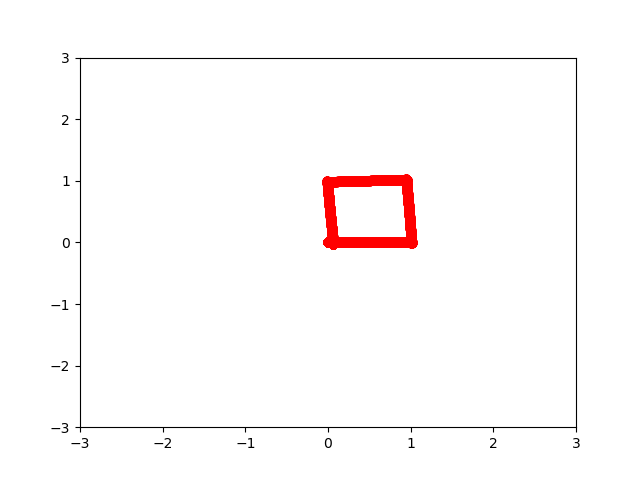
\includegraphics[width=\linewidth]{lab1figure/patrol_plot_1.png}\vspace{-10pt}
            \caption{Plotting the patrol \mintinline{bash}{s 1 1}.}\label{Fig:s_1_1}
          \end{minipage}\hfill
          \begin{minipage}{0.48\textwidth}
            \centering
            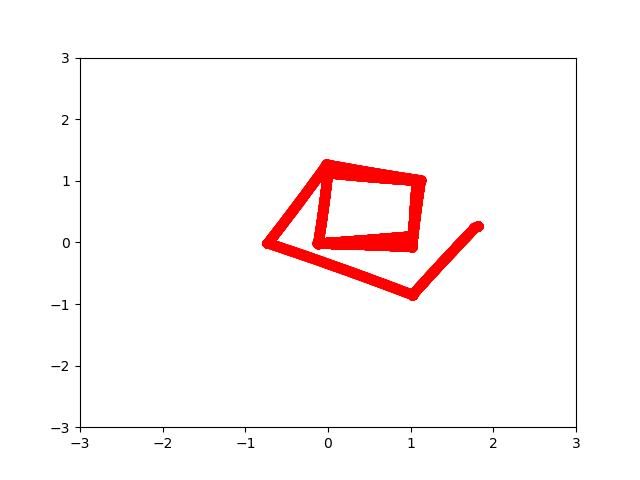
\includegraphics[width=\linewidth]{lab1figure/patrol_plot_2.png}\vspace{-10pt}
            \caption{Plotting the patrol \mintinline{bash}{s 1 2}.}\label{Fig:s_1_2}
          \end{minipage}
       \end{figure}

    \end{enumerate}

    \item Select one of the shapes for patrol, and run it with a number of cycles greater than 1 (e.g. t 1 3). Discuss your observations of accumulation of errors and its impact in the shape of the patrol.
    
    \begin{enumerate}

        \item Before you input the parameters to the client program, open a new terminal and record a rosbag containing the information from relevant topics. You will upload this file with your assignment submission.
        
\begin{minted}{bash}
  $ rosbag record /odom /cmd_vel /tf /scan -O <your_name>_patrol.bag
\end{minted}

        \textbf{Answer: }The required bag file is attached in the submission.
    
        \item Save the x-y plot and include it in your write-up.
        
        \textbf{Answer: }Based on the observation, the error will accumulate as the robot makes more turns and patrols more cycles. At first, it only affects the orientation toward which it walks. But later when it's away from the origin, the path will be so deformed that it looks nothing as planned, and sometimes it hits the wall before completing the patrol.

        \begin{figure}[H]
          \centering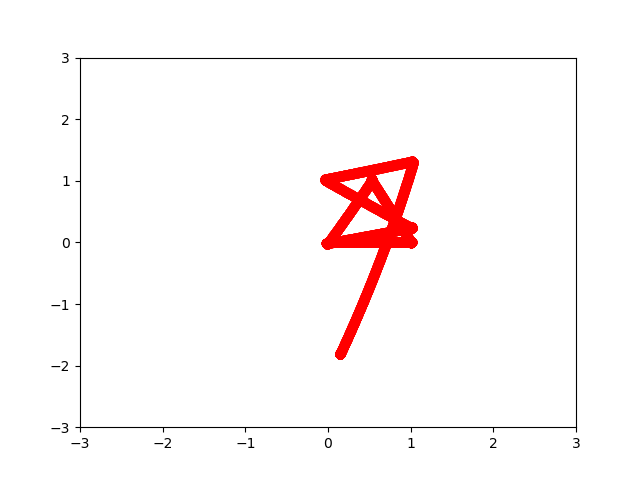
\includegraphics[width=8cm]{lab1figure/patrol_plot_3.png}\vspace{-10pt}
          \caption{Plotting the patrol \mintinline{bash}{t 1 3}.}\label{fig:t_1_3}
          \end{figure}
        
    \end{enumerate}

\end{enumerate}

\end{document}